\documentclass[a4paper,12pt]{article}
\usepackage[utf8]{inputenc}
\usepackage[spanish]{babel}
\usepackage{color}
\usepackage{parskip}
\usepackage{graphicx}
\usepackage{multirow}
\usepackage{listings}
\usepackage{vmargin}
\graphicspath{ {imagenes/} }
\definecolor{mygreen}{rgb}{0,0.6,0}
\definecolor{lbcolor}{rgb}{0.9,0.9,0.9}
\usepackage{epstopdf}


\setpapersize{A4}
\setmargins{2.5cm}       % margen izquierdo
{1.5cm}                        % margen superior
{16.5cm}                      % anchura del texto
{23.42cm}                    % altura del texto
{10pt}                           % altura de los encabezados
{1cm}                           % espacio entre el texto y los encabezados
{0pt}                             % altura del pie de página
{2cm}     

\lstset{
backgroundcolor=\color{lbcolor},
    tabsize=4,    
%   rulecolor=,
    language=SQL,
        basicstyle=\tiny,
        aboveskip={1.5\baselineskip},
        columns=fixed,
        showstringspaces=false,
        extendedchars=false,
        breaklines=true,
        prebreak = \raisebox{0ex}[0ex][0ex]{\ensuremath{\hookleftarrow}},
        frame=single,
        showtabs=false,
        showspaces=false,
        showstringspaces=false,
        identifierstyle=\ttfamily,
        keywordstyle=\color[rgb]{0,0,1},
        commentstyle=\color[rgb]{0.026,0.112,0.095},
        stringstyle=\color{red},
        numberstyle=\color[rgb]{0.205, 0.142, 0.73},
%        \lstdefinestyle{C++}{language=C++,style=numbers}’.
}

\begin{document}

\begin{LARGE}
 CHRISTOFER FABIÁN CHÁVEZ CARAZAS
\end{LARGE}

\textbf{Tiempo promedio de demora: } 2 minutos 30 segundos.

Se tiene los siguientes indices en la tabla Relaciones:

\begin{figure}[h]
 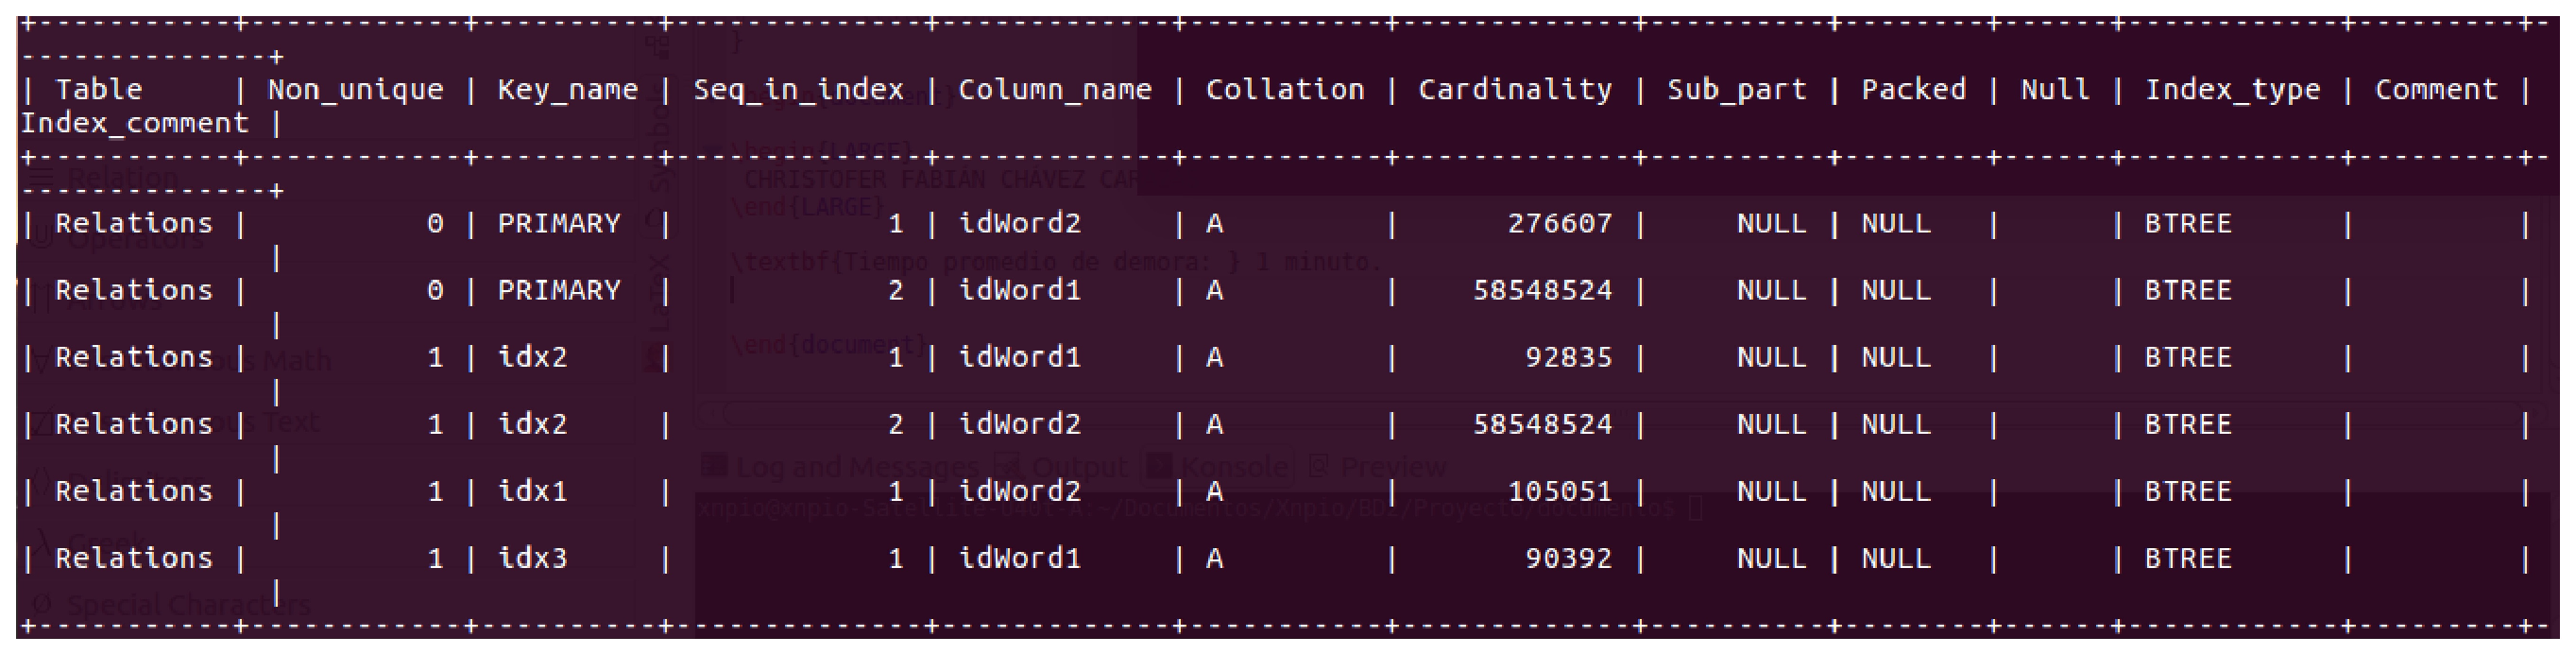
\includegraphics[scale=0.5]{1.eps}
\end{figure}

Un Clustered compuesto, un secundario compuesto y dos secundarios.

Con la siguiente consulta:

\begin{lstlisting}
 select Word, cos from (select X.idWord1, (X.ps/Y.modulo) as cos from 
(select A.idWord1, sum(A.W * B.W) as ps from  Relations  as A inner join  Relations as B on A.idWord2 = B.idWord2 where A.idWord1 <> 1 and B.idWord1 = 1 group by A.idWord1)as X 
inner join (select idWord1, sqrt(sum(W*W)) * (select sqrt(sum(W*W)) from Relations use index(idx2) where idWord1 = 1 group by idWord1)  as modulo from Relations use index(PRIMARY) where idWord1 <> 1 group by idWord1) as Y on X.idWord1 = Y.idWord1) as AA 
inner join Word on idWord1 = idWord order by cos DESC limit 0,10;
\end{lstlisting}


\end{document}
